\section{Модификация проекта «Выпуклая оболочка»}
\subsection*{Точная постановка задачи}
Вычисляется количество вершин выпуклой оболочки, лежащих в 1-окрестности заданного заполненного треугольника.
\subsection*{Решение данной задачи и модификация кода}
Эталонный проект до модификации индуктивно строит выпуклую оболочку по
точкам. При добавлении новой точки программа индуктивно перевычисляет периметр и
площадь оболочки. Наша цель - модифицировать эталонный проект таким 
образом, чтобы вычислялось количество вершин выпуклой оболочки, лежащих в 1-окрестности заданного заполненного треугольника..

Для начала модифицируем файл $\texttt{convex/r2point.rb}$ добавив в класс $\texttt{R2Point}$ методы,
которые выполняют следующие действия:

\medskip
\begin{itemize}
\item нахождение расстояния от точки до отрезка;
\item проверка принадлежности точки треугольнику;
\item проверка принадлежности точки окрестности и треугольнику.
\end{itemize}

\newpage
\begin{small}
\begin{verbatim}
def dist_segm(a,b)
  p1=(@x-a.x)*(b.x-a.x)+(@y-a.y)*(b.y-a.y) 
  p2=(a.x-b.x)*(@x-b.x)+(a.y-b.y)*(@y-b.y)
  return Math.sqrt((@x-a.x)**2+(@y-a.y)**2) if p1<=0 
  return Math.sqrt((@x-b.x)**2+(@y-b.y)**2) if p2<=0 
  a=(a.y-b.y)*@x+(b.x-a.x)*@y+(a.x*b.y-b.x*a.y
  b=Math.sqrt((b.x-a.x)**2+(b.y-a.y)**2)
  return (a/b).abs 
end
\end{verbatim}
\end{small}   

Метод $\texttt{dist\_segm(a,b)}$ основан на векторной алгебре. Первоначально определяется, лежит ли точка левее или правее отрезка, для этого вычисляется скалярное произведение от искомой точки до каждого из карев отрезка.
Если одно из этих скалярных произведений меньше или равно нулю, то возвращается расстояние от точки до края отрезка, скалярное произведение с которым было меньше либо равно нулю, причем считается расстояние как гипотенуза прямоугольного треугольника. Если же скалярные произведения больше нуля, то расстояние считается по формуле, которая указана ниже.
\begin{center}
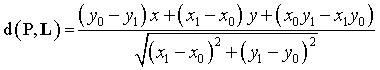
\includegraphics[width=0.5\hsize]{images/distsegm}
\end{center}

\begin{small}
\begin{verbatim}
def inside_triangle?(a,b,c)
  l=(a.x-@x)*(b.y-a.y)-(b.x-a.x)*(a.y-@y)
  m=(b.x-@x)*(c.y-b.y)-(c.x-b.x)*(b.y-@y)
  n=(c.x-@x)*(a.y-c.y)-(a.x-c.x)*(c.y-@y)
  (l>0 && m>0 && n>0) || (l<0 && m<0 && n<0)
end
\end{verbatim}
\end{small} 

Данный метод использует псевдоскалярное произведение для определения, находится ли точка внутри треугольника.
2 вершины треугольника образуют отрезок, который можно воспринять как луч. Этот луч делит всю плоскость на 2 полуплоскости. Берутся 2 вершины треугольника и обозреваемая точка, затем относительно них выполняется псевдоскалярное произведение.

\begin{center}
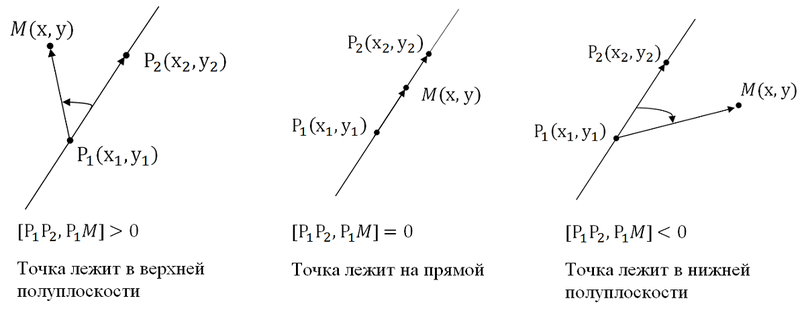
\includegraphics[width=1.1\hsize]{images/psevd}
\end{center}

 Знак числа, которое получается при вычислении говорит нам, в какой из полуплоскостей относительно стороны треугольника лежит точка. Если все знаки чисел, полученных во время вычисления псевдоскалярных произведений относительно всех сторон треугольника, совпадают, значит точка лежит внутри треугольника, иначе, точка находится вне треугольника.

\begin{small}
\begin{verbatim}
def is_inside?(a,b,c)
  return true if self.inside_triangle?(a,b,c) #если в треугольнике
  return true if (self.dist_segm(a,b)<=1 && self.dist_segm(a,b)>=0) ||
  (self.dist_segm(b,c)<=1 && self.dist_segm(b,c)>=0) ||
  (self.dist_segm(c,a)<=1 && self.dist_segm(c,a)>=0) || 
  (self.dist_segm(a,c)<=1 && self.dist_segm(a,c)>=0)
  return false
end
\end{verbatim}
\end{small} 

Метод $\texttt{is\_inside?(a,b,c)}$ выполняет финальную проверку на принадлежность точки треугольнику или окрестности треугольника. Первоначально, он проверяет, лежит ли точка внутри треугольника, вызывая метод $\texttt{inside\_triangle?(a,b,c)}$. Если этот метод вернул true, то и метод $\texttt{is\_inside?(a,b,c)}$ возвращает true, говоря о том, что точка удовлетворяет условию. Если же был получен false, то идет проверка окрестности. Проверяется расстояние от точки до каждой из сторон при помощи метода $\texttt{dist\_segm(a,b)}$. Если хотя бы до одной стороны расстояние больше нуля и меньше единицы, то возвращается true, опять же говоря о том, что точка удовлетворяет условию. Во всех остальных ситуациях (если точка не лежит ни в треугольнике, ни в окрестности) возвращается false, что означает, что точка не удовлетворяет условию и увеличивать количество точек, удовлетворяющих условию, не стоит.

\newpage
Теперь модифицируем файл $\texttt{convex/convex.rb}$. Добавим в класс $\texttt{Figure}$  инициализацию объекта, метод создания треугольника, метод проверки
на принадлежность треугольнику и метод получения количество вершин выпуклой оболочки, которые удовлетворяют нашему условию.

\begin{small}
\begin{verbatim}
def initialize; @ins=0 end
\end{verbatim}
\end{small}

Теперь при инициализации абстрактной фигуры создается переменная экземпляра класса  $\texttt{Figure @ins}$ . Так как в нашем проекте создается только одна выпуклая
оболочка, мы можем использовать именно этот тип переменной.

\begin{small}
\begin{verbatim}
def set_triangle(a,b,c)
  @@a, @@b, @@c = a,b,c
end
\end{verbatim}
\end{small}

Задание треугольника производится тремя точками, которые будут храниться в переменных класса  $\texttt{Figure @@a, @@b, @@c}$ соответственно. Так как при добавлении вершин выпуклой оболочки может произойти создание объекта другого класса, нам придется использовать именно переменные класса, ибо все объекты классов 
$\texttt{Void, Point, Segment, Polygon}$ наследуются от класса $\texttt{Figure}$, а следовательно, наследуют и точки нашего треугольника.

\begin{small}
\begin{verbatim}
def intr?(p) ; (p.is_inside?(@@a,@@b,@@c)) ? 1 : 0 ;end
\end{verbatim}
\end{small}

Метод $\texttt{intr?(p)}$ проверяет принадлежность точки, получаемой в качестве аргумента, заданному ранее треугольнику используя метод $\texttt{is\_inside?(a,b,c)}$, который возвращает true, в случае, если точка лежит 
либо в заданном треугольнике, либо в его единичной окрестности и false во всех остальных случаях. Метод  $\texttt{intr?(p)}$, в случае, если точка попадает в заданный треугольник или его окрестность, возвращает число 1, во всех остальных
случаях он возвращает 0.


\begin{small}
\begin{verbatim}
def inside_points; @ins; end 
\end{verbatim}
\end{small}

Метод $\texttt{inside\_points}$ возвращает переменную экземпляра  $\texttt{@ins}$, которая хранит количесто вершин, лежащих в заданном треугольнике или его единичной окрестности.

Теперь рассмотрим класс  $\texttt{Void}$. Так как объект именно этого класса создается при начале работы программы, то 
задавать треугольник лучше всего именно в нем. Для этого добавим инициализацию объекта класса $\texttt{Void}$.

\begin{small}
\begin{verbatim}
def initialize(a=R2Point.new, b=R2Point.new, c=R2Point.new)
  set_triangle(a,b,c)
end
\end{verbatim}
\end{small}

Если при создании объекта класса $\texttt{R2Point}$ не указать аргументы, то координаты точки будут запрашиваться
через ручной ввод, мы этим воспользуемся. Зададим 3 точки $\texttt{a, b, c}$ и передадим их в метод $\texttt{set\_triangle(a,b,c)}$, чтобы задать эти точки как переменные класса $\texttt{Figure}$, которые в будущем будут
доступны из всех классов.

После задания треугольника можно начать работать с точками выпуклой оболочки. В классе $\texttt{Point}$ изменим 
инициализацию, добавив строчку, которая будет проверять, лежит ли она в заданном ранее треугольнике или его единичной окрестности.

\begin{small}
\begin{verbatim}
class Point < Figure
  def initialize(p) 
    @p = p
    @ins=intr?(@p) 
  end
  ...
end
\end{verbatim}
\end{small}

Если точка удовлетворяет условию, то переменная $\texttt{@ins}$ будет равна 1, в противном случае, она будет равна 0, так как метод $\texttt{intr?(p)}$ возвращает 1, если точка удовлетворяет условию и 0, если не удовлетворяет.

По тому же принципу изменим инициализацию класса $\texttt{Segment}$ и класса $\texttt{Polygon}$

\begin{small}
\begin{verbatim}
class Segment < Figure
  def initialize(p, q) 
    @p, @q = p, q
    @ins=intr?(@p)+intr?(@q)
  end
  ...
end

class Polygon < Figure
  attr_reader :points, :perimeter, :area 
  ...
  @area      = R2Point.area(a, b, c).abs
  @ins=intr?(a)+intr?(b)+intr?(c)
  end
\end{verbatim}
\end{small}




Также нам нужно будет проверить пересекаются ли прямые, на которых лежит ребро выпуклой оболочки и 
заданный отрезок. Для этого добавим в файл $\texttt{convex/convex.rb}$ метод $\texttt{cross?}$ в класс 
$\texttt{Segment}$, который будет проверять данное условие.

\begin{small}
\begin{verbatim}
def cross?(point1,point2)
 if (point1.x==point2.x && self.p.x==self.q.x)
  return false
 else
  an=(point2.y-point1.y)/(point2.x-point1.x)
  bn=(self.q.y-self.p.y)/(self.q.x-self.p.x)
  if an == bn
   return false
  else
   return true
  end
 end
end
\end{verbatim}
\end{small}

Ещё нам необходимо проверить является ли найденная точка пересечением прямых или точкой пересечения отрезков. 
Чтобы этот случай учитывался добавим в файл $\texttt{convex/convex.rb}$ метод $\texttt{is\_on\_segments?}$ в 
класс $\texttt{Segment}$.


\begin{small}
\begin{verbatim}
def is_on_segments?(point1,point2)
 j=crosspoint(point1,point2).inside?(point1,point2)
 k=crosspoint(point1,point2).inside?(@p,@q)
 if cross?(point1,point2)
  j and k
 else
  false
 end
end
\end{verbatim}
\end{small}

Теперь можно приступить к созданию нового метода, который будет вычислять периметр части ребра, лежащего 
внутри или на границе заданного треугольника. Для этого создадим новый метод $\texttt{part\_perimeter}$ 
и добавим его в класс $\texttt{Segment}$.

Для начала проверим с помощью метода $\texttt{outside\_tr?}$ лежат ли обе точки отрезка внутри или на границе треугольника (рис.1). 
\newpage\begin{figure}[ht!]
\begin{center}
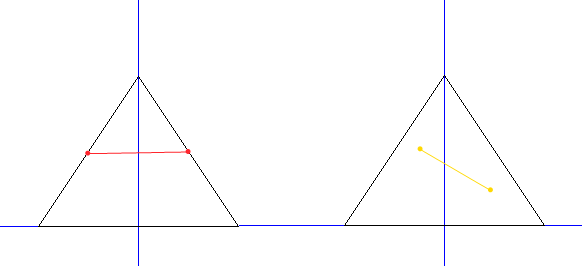
\includegraphics[width=0.8\hsize]{images/1}
\end{center}
\caption{}\label{fig:convex}
\end{figure}


Если точки лежат, то возвращаем расстояние от одной точки до другой как периметр. Для этого используем метод $\texttt{dist}$, который вычисляет расстояние по формуле:

$$\sqrt{(x_2-x_1)^2+(y_2-y_1)^2}_.$$

Если точки не лежат, то продолжаем проверку. Проверяем следующее условие, когда одна точка лежит снаружи, а другая находится строго внутри треугольника, 
тогда вычисляем расстояние от точки пересечения одной из сторон треугольника до точки лежащей строго внутри треугольника. Для нахождения точки пересечения используем метод  
$\texttt{crosspoint}$ и выводим расстояние от найденой точки до точки лежащей строго внутри треугольника. 

Если одна точка строго снаружи, а другая точка лежит на границе треугольника, тогда проверяем лежит ли 
одна точка на отрезке, а другая на прямой с помощью методов $\texttt{on\_segment? и on\_line?}$. Также необходимо учитывать,
что обе точки могут лежать на одной прямой (рис. 2). Тогда выводим расстояние прямой лежащей в треугольнике или на его границе.
\begin{figure}[ht!]
\begin{center}
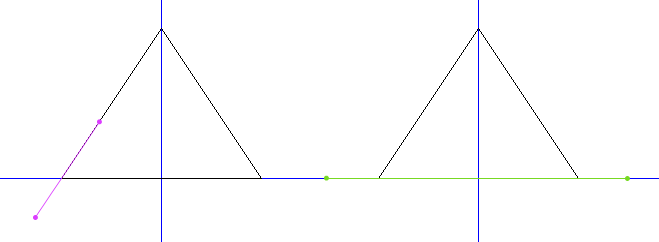
\includegraphics[width=0.8\hsize]{images/2}
\end{center}
\caption{}\label{fig:convex}
\end{figure}

Для метода $\texttt{is\_on\_segments?}$ создадим массив куда будем добавлять результат, является ли найденная точка 
пересечения прямых $-$ точкой пересечения отрезков.
И выводим расстояние от одной точки до другой. 

После рассмотренных случаев метод $\texttt{part\_perimeter}$ примет следующий вид:
\begin{small}
\begin{verbatim}
class Segment < Figure
  ...
def part_perimeter()
  pt=!@p.outside_tr?(@point1,@point2,@point3)
  pt=!@q.outside_tr?(@point1,@point2,@point3)
  pq=@p.outside_tr?(@point1, @point2, @point3)
  qp=@q.inside_tr?(@point1, @point2, @point3)
  pv=@q.outside_tr?(@point1, @point2, @point3)
  qv=@p.inside_tr?(@point1, @point2, @point3)
  
  if pt and pt
    return @p.dist(@q)                         
  elsif pq and qp
    if is_on_segments?(@point1, @point2) 
	  return @p.dist(@q) - crosspoint(@point1, @point2).dist(@p)
	elsif is_on_segments?(@point2, @point3)
	  return @p.dist(@q) - crosspoint(@point2, @point3).dist(@p) 
    elsif is_on_segments?(@point1, @point3)
	  return @p.dist(@q) - crosspoint(@point1, @point3).dist(@p)  
	end
  elsif pv and qv
    if is_on_segments?(@point1, @point2) 
	  return @p.dist(@q) - crosspoint(@point1, @point2).dist(@q) 
    elsif is_on_segments?(@point2, @point3)
	  return @p.dist(@q) - crosspoint(@point2, @point3).dist(@q) 
    elsif is_on_segments?(@point1, @point3)
	  return @p.dist(@q) - crosspoint(@point1, @point3).dist(@q) 
	end
  else
    if @q.on_segment?(@point1, @point2) && @p.on_line?(@point1, @point2)
      return @p.dist(@q) - [@p.dist(@point1), @p.dist(@point2)].min
    elsif @q.on_segment?(@point2, @point3) && @p.on_line?(@point3, @point2)
      return @p.dist(@q) - [@p.dist(@point3), @p.dist(@point2)].min
    elsif @q.on_segment?(@point1, @point3) && @p.on_line?(@point3, @point1)
      return @p.dist(@q) - [@p.dist(@point3), @p.dist(@point1)].min
    end
	  
      if @p.on_segment?(@point1, @point2) && @q.on_line?(@point1, @point2)
        return @p.dist(@q) - [@q.dist(@point1), @q.dist(@point2)].min
      elsif @p.on_segment?(@point2, @point3) && @q.on_line?(@point3, @point2)
        return @p.dist(@q) - [@q.dist(@point3), @q.dist(@point2)].min
      elsif @p.on_segment?(@point1, @point3) && @q.on_line?(@point3, @point1)
        return @p.dist(@q) - [@q.dist(@point3), @q.dist(@point1)].min
      end
	  
	  
	  
      if @p.on_line?(@point1, @point2) && @q.on_line?(@point1, @point2)
	     return @point1.dist(@point2) 
      elsif @p.on_line?(@point3, @point2) && @q.on_line?(@point3, @point2)
	    return @point3.dist(@point2) 
      elsif @p.on_line?(@point1, @point3) && @q.on_line?(@point1, @point3)
	    return @point1.dist(@point3) 
	  end
	  
      array = []
	  
	  if is_on_segments?(@point1, @point2)
	    array << crosspoint(@point1, @point2) 
      elsif is_on_segments?(@point2, @point3)
	    array << crosspoint(@point2, @point3) 
      elsif is_on_segments?(@point1, @point3)
	    array << crosspoint(@point1, @point3) 
	  end
	  
      if array.size == 3 
       if array[0] != array[1]
	     return array[0].dist(array[1]) 
       elsif array[2] != array[1]
	     return array[2].dist(array[1]) 
       elsif array[0] != array[2]
	     return array[0].dist(array[2]) 
	   end
      elsif array.size == 2
        return array[0].dist(array[1])
      else
        return 0.0
      end
    end
  end
	...
end
\end{verbatim}
\end{small}

Также нам необходимо модифицировать класс $\texttt{Polygon}$, добавив небольшие изменения в методы 
$\texttt{initialize и add(t)}$, а именно:
 
Вычисляем периметр части выпуклой оболочки лежащей в заданном треугольнике.
\begin{small}
\begin{verbatim}
class Polygon < Figure
  attr_reader :points, :perimeter, :area, :part_perimeter
  ...
  def initialize(a, b, c, point1, point2, point3) 
    ...
    ao=Segment.new(a, b, @point1, @point2, @point3).part_perimeter
    bo=Segment.new(b, c, @point1, @point2, @point3).part_perimeter
    co=Segment.new(a, c, @point1, @point2, @point3).part_perimeter
    @part_perimeter = ao + bo + co;  end
\end{verbatim}
\end{small}	  
Когда добавляем новую точку нужно рассмотреть несколько случаев:
\begin{enumerate}
\item если освещённых ребер нет, что означает новая точка попала внутрь или 
  на границу старой выпуклой оболочки и нам нечего не нужно делать;
\item если хотя бы одно освещённое ребро есть, то их нужно удалить и соединить концы оставшейся ломаной с новой точкой.
\end{enumerate}
\begin{small}
\begin{verbatim}
 def add(t)
   ...
  if t.light?(@points.last, @points.first)
    ...
  dl=Segment.new(@points.first,@points.last,@point1,@point2,@point3)
  @part_perimeter -= dl.part_perimeter
    ...
\end{verbatim}
\end{small}	
Для каждого освещённого ребра нам нужно уменьшить периметр оболочки на его длину.
\begin{small}
\begin{verbatim}
  while t.light?(p, @points.first)
    ...
  det=Segment.new(@points.first, p, @point1, @point2, @point3).part_perimeter
  @part_perimeter -= det
    ...
  end
  ...

  while t.light?(@points.last, p)
   ...
   get=Segment.new(p, @points.last, @point1, @point2, @point3).part_perimeter
   @part_perimeter -= get
   ...
  end
\end{verbatim}
\end{small} 
Затем нам необходимо добавить сумму длин двух новых рёбер.
\begin{small}
\begin{verbatim}
       ... 
    ml=Segment.new(@points.first, t, @point1, @point2, @point3).part_perimeter
    nl=Segment.new(t, @points.last, @point1, @point2, @point3).part_perimeter
    @part_perimeter += ml + nl
    ...
   end
   self
  end
end
\end{verbatim}
\end{small}

Но для того чтобы рисовался треугольник нам нужно модифицировать файл $\texttt{convex/tk\_drawer.rb}$ 
метод $\texttt{draw}$ класса $\texttt{Figure}$:
\begin{small}
\begin{verbatim}





class Figure
  def draw
   ...
    TkDrawer.draw_line(@point1, @point2)
    TkDrawer.draw_line(@point2, @point3)
    TkDrawer.draw_line(@point3, @point1)
  end
end
\end{verbatim}
\end{small}

Для вывода результата на экран изменяем в файлах $\texttt{convex/run\_tkconvex.rb}$ и $\texttt{convex/run\_convex.rb}$ несколько строк.


\begin{small}
\begin{verbatim}
  fig = Void.new(R2Point.new, R2Point.new, R2Point.new)
    ...
  puts "S = #{fig.area}, P = #{fig.perimeter} perimetr = #{fig.part_perimeter}"
\end{verbatim}
\end{small}

Модификация эталонного проекта «Выпуклая оболочка» завершена. Пример работы программы можно увидеть на (рис.3).

\begin{figure}[ht!]
\begin{center}
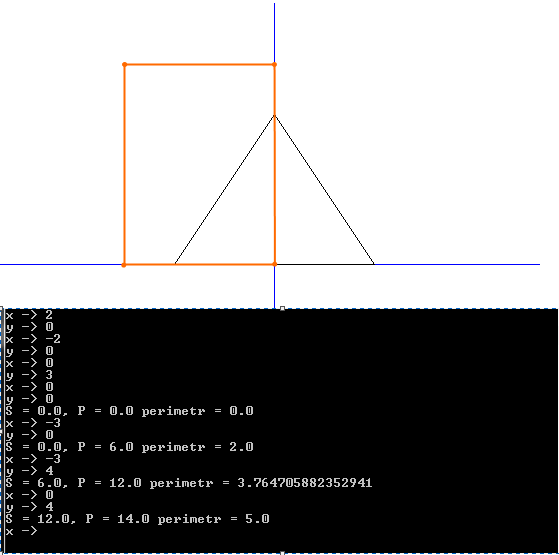
\includegraphics[width=0.8\hsize]{images/3}
\end{center}
\caption{Работа программы «Выпуклая оболочка»}\label{fig:convex}
\end{figure}












